\subsection{设计与主要比较}
\label{sec:f2-admission}
六构建器、三种子研究交叉策略强制与门控：II-A（自由、无门控）、II-B（自由、门控）、II-C（强制、无门控）、II-D（强制、门控）。强制策略来自固定集合，自由构建器在附录~\ref{app:free-vocabulary} 的词汇中选择声明。评估使用九个数据库的 $1{,}169$ 题、官方 BIRD 评分器，并包含已披露的 $18$ 题冒烟例外。下列结果来自对结果前规格的校正重分析。

\begin{table}[H]
\centering\small
\begin{tabular}{@{}lrr@{}}
\toprule
Metric & II-A & II-D \\
\midrule
Candidate count & 5.78 & 3.83 \\
Oracle accuracy (\%) & 76.14 & 75.70 \\
Best-fixed accuracy (\%) & 67.58 & 67.30 \\
Headroom (pp) & 8.56 & 8.40 \\
\midrule
D$-$A headroom (pp) & \multicolumn{2}{c}{$\RevisionPrimaryDelta$} \\
Unadjusted bootstrap 95\% CI & \multicolumn{2}{c}{$\RevisionPrimaryCI$} \\
One-sided sign-flip $p$ & \multicolumn{2}{c}{$\RevisionPrimaryP$} \\
\bottomrule
\end{tabular}

\caption{\textbf{校正后的主分析。}数值为 $1{,}169$ 个问题上 $18$ 个构建器–种子单元格的均值；\bare{} 同时计入 oracle 与最佳固定对照。}
\label{tab:primary}
\end{table}

强制／门控减自由／无门控的含基线 oracle 余量对比为 $\RevisionPrimaryDelta$\,pp，单元对比范围 $\RevisionPrimaryRange$\,pp。实际组合政策未提高观测平均余量；不确定性见表~\ref{tab:primary}。

\begin{figure}[H]
\centering
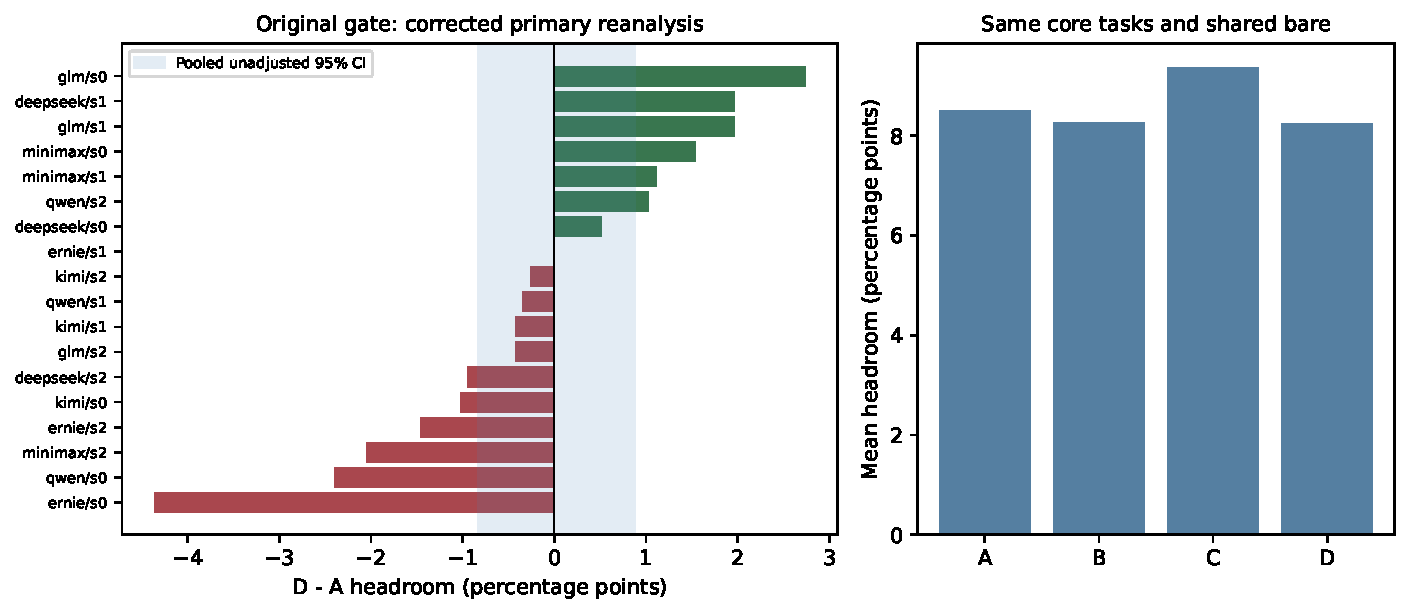
\includegraphics[width=0.72\linewidth]{figures/fig_results_revision.pdf}
\caption{\textbf{版本化校正重分析。}左：完整集合的 D$-$A 单元格对比与合并 95\% 区间。右：共享核心 400 题上、以共同 \bare{} 为基线的四臂余量。}
\par\smallskip{\footnotesize 图中余量和差值坐标均表示百分点。}
\label{fig:results}
\end{figure}

核心 $400$ 题的门控对比为 $\RevisionGateDelta$\,pp，策略与交互效应尚无定论（表~\ref{tab:factorial}）；固定 $K$ 对比为 $\RevisionKmatchedDelta$\,pp。II-E 仍仅用于开发。R2/R3 审核（附录~\ref{app:r2}）为这些单次覆盖测量提供参照：R2 翻转 $8.54\%$，三次运行间 $14.5\%$ 的基线题目改变正确性，同代码 oracle 缺口为 $6.50$\,pp。

\begin{table}[H]
\centering\small
\begin{tabular}{@{}lrrrr@{}}
\toprule
Contrast & Effect (pp) & 95\% CI (pp) & Raw $p$ & Holm $p$ \\
\midrule
Gate & $-0.69$ & $[-1.56, +0.20]$ & 0.026 & 0.079 \\
Strategy & $+0.42$ & $[-0.32, +1.51]$ & 0.263 & 0.428 \\
Interaction & $-0.87$ & $[-2.83, +0.65]$ & 0.214 & 0.428 \\
\bottomrule
\end{tabular}

\caption{\textbf{校正后的核心 400 题析因重分析。}门控为 $[(B{-}A)+(D{-}C)]/2$，策略为 $[(C{-}A)+(D{-}B)]/2$，交互为 $(D{-}C)-(B{-}A)$；给出原始与 Holm 调整 $p$ 值。}
\label{tab:factorial}
\end{table}
